% ch04-model-entailment.tex — Models and Entailment
% Shows multiple interpretations, which are models of O, and entailment as
% "true in ALL models". Pedagogical purpose: make O ⊨ α visually intuitive.
\documentclass[tikz,border=5pt]{standalone}
\usepackage{fontspec}
\setmainfont{Times New Roman}
\usepackage{unicode-math}
\setmathfont{Cambria Math}
\usetikzlibrary{shapes.geometric,positioning,fit,backgrounds,arrows.meta,decorations.pathreplacing}

\begin{document}
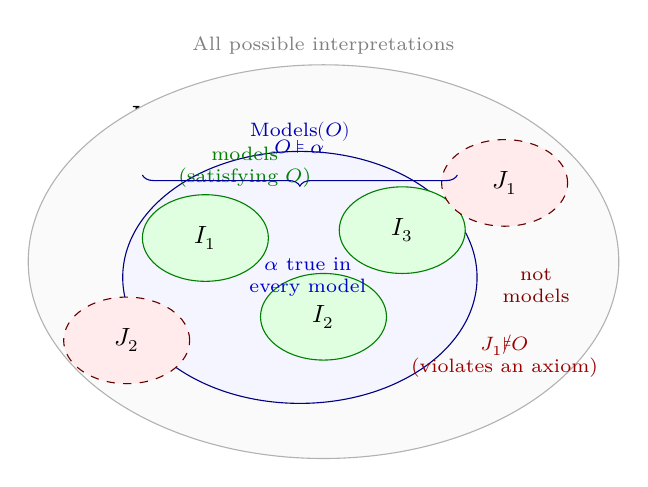
\begin{tikzpicture}[
  interp/.style={ellipse,draw,minimum width=1.6cm,minimum height=1.1cm,
                 font=\small,inner sep=2pt},
  modelyes/.style={interp,fill=green!12,draw=green!50!black},
  modelno/.style={interp,fill=red!8,draw=red!40!black,dashed},
  labelstyle/.style={font=\scriptsize,align=center},
]

% Title
\node[font=\small\bfseries,anchor=north] at (3.5,3.6)
  {Models and Entailment: $O \models \alpha$};

% All interpretations universe
\node[ellipse,draw=black!30,minimum width=7.5cm,minimum height=5cm,
      fill=black!2,label={[font=\scriptsize,gray]north:All possible interpretations}] (universe) at (3.5,1.5) {};

% Models of O (subset)
\node[ellipse,draw=blue!50!black,minimum width=4.5cm,minimum height=3.2cm,
      fill=blue!4,label={[font=\scriptsize,text=blue!70!black]north:$\mathrm{Models}(O)$}] (models) at (3.2,1.3) {};

% Individual interpretations
\node[modelyes] (I1) at (2.0,1.8) {$I_1$};
\node[modelyes] (I2) at (3.5,0.8) {$I_2$};
\node[modelyes] (I3) at (4.5,1.9) {$I_3$};
\node[modelno]  (J1) at (5.8,2.5) {$J_1$};
\node[modelno]  (J2) at (1.0,0.5) {$J_2$};

% Labels for models vs non-models
\node[labelstyle,text=green!50!black] at (2.5,2.7) {models\\(satisfying $O$)};
\node[labelstyle,text=red!50!black] at (6.2,1.2) {not\\models};

% α annotation
\node[font=\scriptsize,align=center,text=blue!80!black] at (3.3,1.3)
  {$\alpha$ true in\\every model};

% Brace pointing to models
\draw[decorate,decoration={brace,amplitude=4pt,mirror},blue!60!black]
  (1.2,2.6) -- (5.2,2.6)
  node[midway,above=4pt,font=\scriptsize,text=blue!70!black]{$O \models \alpha$};

% Non-model note
\node[font=\scriptsize,text=red!60!black,align=center] at (5.8,0.3)
  {$J_1 \not\models O$\\(violates an axiom)};

\end{tikzpicture}
\end{document}
